%!TEX root = doc.tex
\section{Solution Proposal} % (fold)
\label{sec:proposal}

RepACL's implementation of the FIPA interaction protocols is essentially JADE-inspired. JADE's approach consists of using behaviors for the agents that take the role of initiator or responder and provide be basic functionality of each protocol, allowing the programmer to implement his own handlers for the messages while maintaining all the communication logic behind the scenes.

As figure \ref{fig:arch} illustrates, many concepts from JADE were ported to RepACL. The agent class contains a queue of behaviors and a mail box. The protocol package contains the implementation of different FIPA protocols, namely the AchieveRE ´´request-like´´ protocol, propose, and contract net. Other protocols can be created by extending these or creating entire new behaviors by extending the super class Behavior.

\begin{figure}[h]
	\centering
	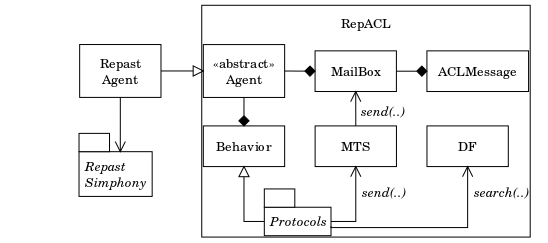
\includegraphics[width=0.5\textwidth]{figures/repacl_arch.png}
	\caption{Detailed architecture or RepACL}
	\label{fig:arch}
\end{figure}

% section proposal (end)